\subsection{The global condition can fail on valid finite-grid inputs}
\label{sec:finite-grid-counterexamples}
A universal prior-support restriction and a statement about typical data are different claims.  The distinction persists after clipping at the training margin, even for a network that fits all training examples with substantial margin.  Our strongest example is an ordinary minibatch-SGD tanh network of hidden depth 16 and width 256, trained on all 60,000 MNIST images for even-versus-odd classification.  It has $98.92\%$ empirical test accuracy, and a separate exact computation verifies every signed training output above $4.4815762$.  The finite-radius counterexample below is independently verified.  The saved weights are used without rescaling.

The left image in Figure~\ref{fig:finite-grid-counterexamples} is a valid $28\times28$ eight-bit grayscale input.  At the smallest tested radius constant $c=10^{-3}$, its clean and disturbed real outputs are enclosed around
\[
 -0.00162845134\longmapsto-0.15496440197.
\]
The resulting score change exceeds $0.15333>1/16$ after clipping at either $1/2$ or $1$.  The image has a black two-pixel border, mean ink $0.17200$, and $64.2\%$ black pixels.  It is a synthetic off-data image, not an image to which we assign a natural digit label.  Its pixel $p_j$ is interpreted as the exact rational input $x_j=2p_j/255-1$; we also independently checked the same witness under the original float32 pixel preprocessing used for training.

The disturbance budget was checked using exact integer-rational arithmetic, and the two network evaluations used 100-decimal outward interval arithmetic with the saved dyadic weights.  In particular,
\[
 (1+H E_v)\left(N^{-1}\sum_{s=1}^{H}\|\eta_s\|_2^2+\xi^2\right)
 <10^{-6}.
\]
The intervals verify that every perturbed hidden coordinate remains in $[-1,1]$: their absolute values are all below $0.061110$.  Thus requiring disturbances to leave activations within their original range does not remove this counterexample.  Its scalar output disturbance has absolute value below $7.3\times10^{-10}$.  Removing it decreases the noise budget and changes either clipped score by at most that amount, so hidden disturbances alone still give a violation.  These are finite-radius witnesses, rather than conclusions drawn only from a large Jacobian or from an unverified optimization output.  They trust the interval-arithmetic implementation and are not Lean formalizations.

The right image provides a second example in a depth-32, width-128 SGD model for MNIST 3 versus 8, with test accuracy $99.09\%$.  Its output changes from $-0.0034068096$ to $-0.3168576499$ at the same $c=10^{-3}$, a clipped-score change greater than $0.31345$.  All perturbed hidden coordinates have absolute value below $0.128211$.  This second model has three training errors, so it is evidence about the naturalness of a support restriction rather than an additional example in the exact training-likelihood event.  A related near-gray eight-bit witness for this model has score change greater than $0.30799$.  The low-ink examples exclude an explanation specific to a uniformly gray background, while remaining clearly off-data.

Each exploratory search had a fixed budget declared before that search.  For the low-ink examples we solved an ink-minimizing linear program, subject to zero first preactivations and a black border, generated 4,096 stochastic roundings to the pixel grid using a fixed seed, and attacked the 16 candidates with smallest absolute clean output.  We then verified selected witnesses independently.  This protocol proves existence, not the prevalence of instability under the data distribution.  In separate probes preserving empirical one-pixel foreground probabilities and on interpolations of opposite-class test images, some violations were verified at $c=10^{-2}$; failure to find violations at smaller radii was not treated as a certificate.

\begin{figure}[t]
\centering
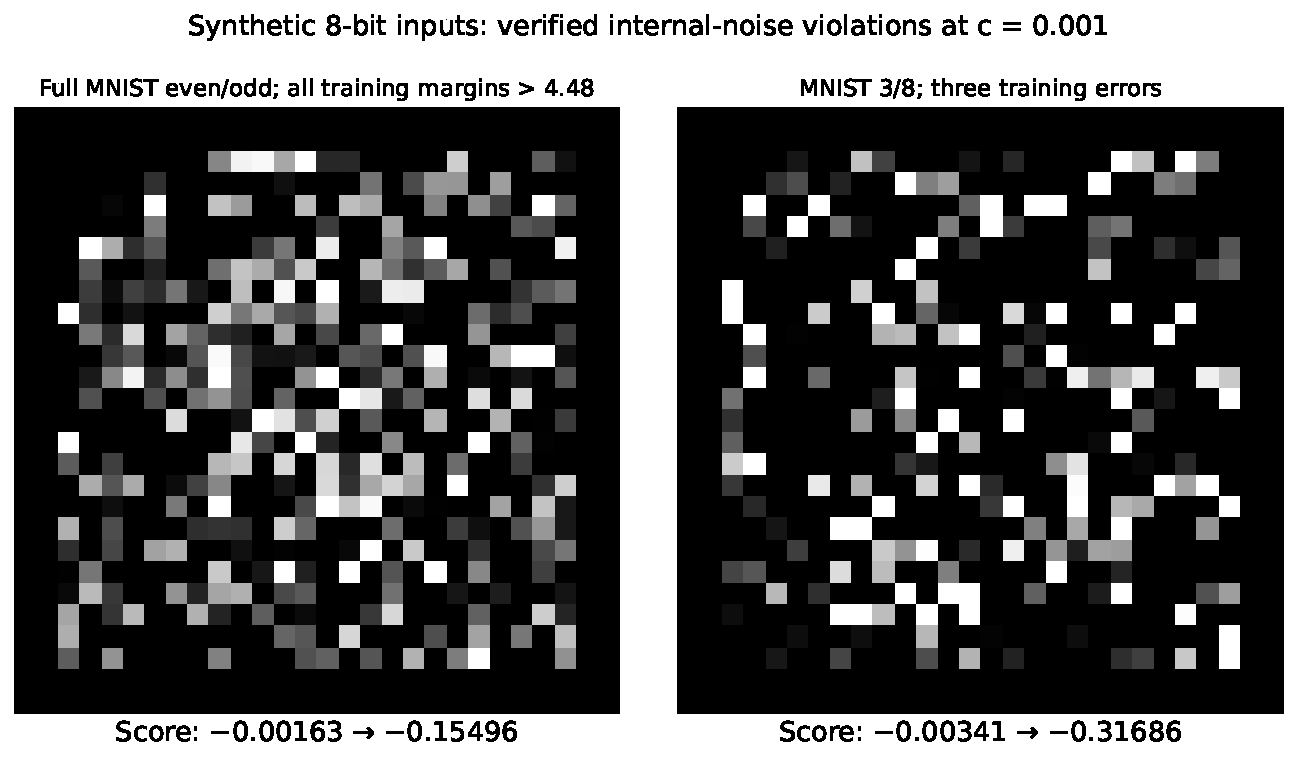
\includegraphics[width=.98\linewidth]{certificates/finite-grid-counterexamples.pdf}
\caption{Synthetic, valid eight-bit inputs violating the global clipped-score condition at $c=.001$.  Both have a fixed black border and low total ink.  The left network was trained on the full MNIST even-versus-odd task and has exactly verified training margins above $4.4815762$; the right network was trained on digits 3 and 8.  The images themselves are unchanged by the internal disturbances.  These are off-data counterexamples, not mislabeled examples from a test set.}
\label{fig:finite-grid-counterexamples}
\end{figure}

\paragraph{A precise Boolean interpretation.}
The finite-grid issue is not inherently a continuous-input phenomenon.  Write each pixel in bits $p_j=\sum_{b=0}^7 2^b q_{jb}$, with $s_{jb}=2q_{jb}-1\in\{-1,1\}$.  Since $\sum_b2^b=255$,
\[
 \frac{2p_j}{255}-1=\sum_{b=0}^7\frac{2^b}{255}s_{jb}.
\]
Replacing row $j$ of the first-layer matrix by eight rows $(2^b/255)W_{0,j}$ gives a network on $8\cdot784=6272$ Boolean inputs with exactly the same outputs, hidden trajectories, readout energy, and internal-noise budgets.  Its depth and width are unchanged.  Thus every rational-pixel witness is also an exact Boolean-input witness for this linearly decoded network.  With the usual dimension-weighted first-layer Frobenius energy, the non-bias weight contribution grows only by
\[
 8\sum_{b=0}^7(2^b/255)^2
 =\frac{8(4^8-1)}{3\cdot255^2}<2.69.
\]
The first-layer bias is unchanged but its dimension weight grows eightfold.  Consequently total first-layer energy, including the bias, increases by at most a factor of eight.
This equivalence uses exact rational pixel normalization.  The software used to train and evaluate the original model normalizes pixels in float32; the original-preprocessing witnesses were checked separately, and the held-out empirical audits use precisely those float32-normalized inputs.  We do not identify the two normalization maps as exact equalities.

\paragraph{An optional margin-band score.}
As a separate, post-protocol comparison, consider
$U(z)=\operatorname{sign}(z)\min\{1/4,(|z|-1/4)_+\}$, which ignores changes entirely inside the already-failing test-margin band.  The original depth-32 low-ink witness still violates its $1/16$ condition, with $U$-score change greater than $0.0668576$; its near-gray witness does not.  For the fitted full-MNIST depth-16 model, the zero-centered witness lies entirely within the ignored band.  We therefore declared a new, explicitly variant-specific exploratory protocol: move the continuous low-ink input toward clean output $3/8$, generate 4,096 pixel-grid roundings, retain the 16 closest to $3/8$, and apply the same internal-noise attack budget.  The independently verified witness has
\[
 z=0.3628586342\longmapsto0.5158098496,
 \qquad |\Delta U|>0.1371413>1/16
\]
at $c=.001$.  All disturbed hidden coordinates have absolute value below $0.089882$.  Here too the scalar output disturbance is below $7.3\times10^{-10}$, so the same $1$-Lipschitz argument gives a hidden-disturbance-only violation.  This secondary result shows that the weaker score can move the fragile input region without eliminating the global obstruction; it does not change the primary clipped-score protocol.

The predeclared longer-training check also supplies a depth-$32$ example.  Of the two fixed continuations, model \texttt{301} fits all $11{,}982$ training examples with minimum signed output above $2.4106$ and achieves $99.24\%$ held-out accuracy.  A valid low-ink, black-border 8-bit image has interval-verified output change $-.00895437\mapsto+.30415992$ at $c=.001$, hence clipped-score change exceeding $.31311$.  Every noisy hidden state remains in $[-1,1]$.  The other continuation retains three training errors; both outcomes and both prescribed searches are retained.  Training metrics in this paragraph are ordinary float64 evaluations, whereas the displayed counterexample has an exact rational noise-budget check and outward interval forward evaluation.

A still weaker, exploratory implication-only condition asks that, for both labels $y$, $yz\ge1/2$ imply $yz^\eta\ge7/16$, and $yz\le1/4$ imply $yz^\eta\le5/16$.  Negating the already saved perturbation for model \texttt{301}, without any new optimization or input selection, yields the interval-verified output $-.32205298$ from the same clean value $-.00895437$.  With $y=-1$, the second implication fails.  Its margin-band score also changes by more than $.07205>1/16$.  The exact noise budget is unchanged by negation and every disturbed hidden state remains in $[-1,1]$.  This auxiliary check concerns later proposed variants; it does not change the primary score convention or empirical protocol.

\paragraph{Failure starting from a confident output.}
A further, separately declared finite-budget check targets clean output $.55$ in the fitted full-MNIST model \texttt{105}.  The resulting valid eight-bit, low-ink input has independently replayed interval enclosures around
\[
 z=0.539345460246\longmapsto z^\eta=0.386611305539
 \qquad(c=.001).
\]
Here the scalar output disturbance is exactly zero.  The exact rational hidden-noise budget passes, and every disturbed hidden coordinate has absolute value below $.101215$.  Thus the first implication above fails for $y=+1$: a clean signed output above $1/2$ falls below $7/16$.  Both the clipped score and the optional margin-band score change by more than $.113388>1/16$.  The same saved disturbance was independently verified under the original float32 pixel preprocessing.  The input is synthetic and has no assigned digit label; the positive clean output establishes the implication's premise.  This check refutes an explanation of the observed instability based solely on clean outputs near zero.  It does not show that this image model satisfies the original all-input clean-margin restriction, which its other near-zero inputs already violate.
